% section
\section{Introduction} \label{section::introduction}
 The task of this chapter is to give the reader the basic knowledge, which is necessary to follow the rest of the thesis. In general, the reader should have basic 
 knowledge about machine learning and neural networks.
 As this thesis is in the field of machine learning, more explicit neural networks and image-/video-prediction, this chapter will start giving basic knowledge about image-/video-prediction
 and specific neural network architectures, which are used in the thesis.\\\\
 The necessary neural network architectures are Autoencoder~\ref{subsection::autoencoder}, CNN~\ref{subsection::cnn} RNN~\ref{subsection::rnn}, 
 LSTM~\ref{subsection::lstm} and ConvLSTM~\ref{subsection::convlstm}, they are described briefly for the reader.
 Afterwards I describe the backpropagation algorithm~\ref{subsection::backpropagation} and BPTT~\ref{subsection::bptt} at a very basic level.
 Those two algorithms are the most used algorithms in training neural networks and are used in this thesis.

 % subsection
 \subsection{Image-Prediction / Video-Prediction} \label{subsection::imageprediction}
  Image-/Video-prediction is a field inside machine learning, where the key is to predict future images, given a sequence of images. The image sequence $X$ is of 
  length $n$, ($x_0, \ldots, x_{n-1}$).
  \\\\
  One possible use-case is the \textbf{one-frame prediction}, where one predicts $x_n$, given the the sequence $X$. Another common use-case is \textbf{multi-frame prediction}, where the key is to 
  predict $t > 1$ many frames into the future ($x_n, \ldots, x_{n+t-1}$).
  This is often performed using sequence-to-sequence learning \cite{Sutskever2014}. The first frames will look much better then the last frames, as 
  ground-truth is missing, The predicted frames are only approximated, which means they contain a certain level of error, so using them as input to perform \textbf{multi-frame prediction} will
  increase the level of error for the following frames.

 % subsection
 \subsection{Autoencoder} \label{subsection::autoencoder}
  The autoencoder is a network architecture, which consists of two neural networks chained together. The first network is called Encoder. This Encoder gets the input $x$ and outputs
  the code h. Often the output layer of the Encoder is named bottleneck-layer. The second network is called Decoder. It gets the code $h$ as input
  and outputs $x \prime$. This architecture is used for reconstruction, where $x \approx x \prime$. To prevent the architecture to simply copy the input directly to the output (which would be an
  interpolation and not the goal of any machine learning algorithm.), there are different techniques to have the autoencoder to instead approximate the output.
  \begin{equation}
   E(x) = h
  \end{equation}
  \begin{equation}
   D(h) = x \prime
  \end{equation}
  The simplest autoencoder architecture is the so named undercomplete autoencoder \cite{Goodfellow2016}, in which the output of the bottleneck-layer $h$ is smaller then the input $x$.
  Therefore the architecture needs to learn how to extract useful features from the input $x$, because it is not able to simply copy the input $x$ to the output $x \prime$, because $h$ is a reduced
  representation of $x$.
  For example a undercomplete convolutional autoencoder, which is just the autoencoder architecture using convolutional layer, gets an input image, which it 
  should reconstruct.
  If the code is smaller then the input image, the network needs to abandon information from the input. The idea is, that during the training, the network learns
  what type of information is obsolete and what type of information is necessary and should be stored in the code, to get a useful approximated $x \prime$.  
  There are many different ideas of using the autoencoder architecture, which are described more in-depth in e.g. Goodfellow et. al. \cite{Goodfellow2016}.
  \begin{figure}[H]
   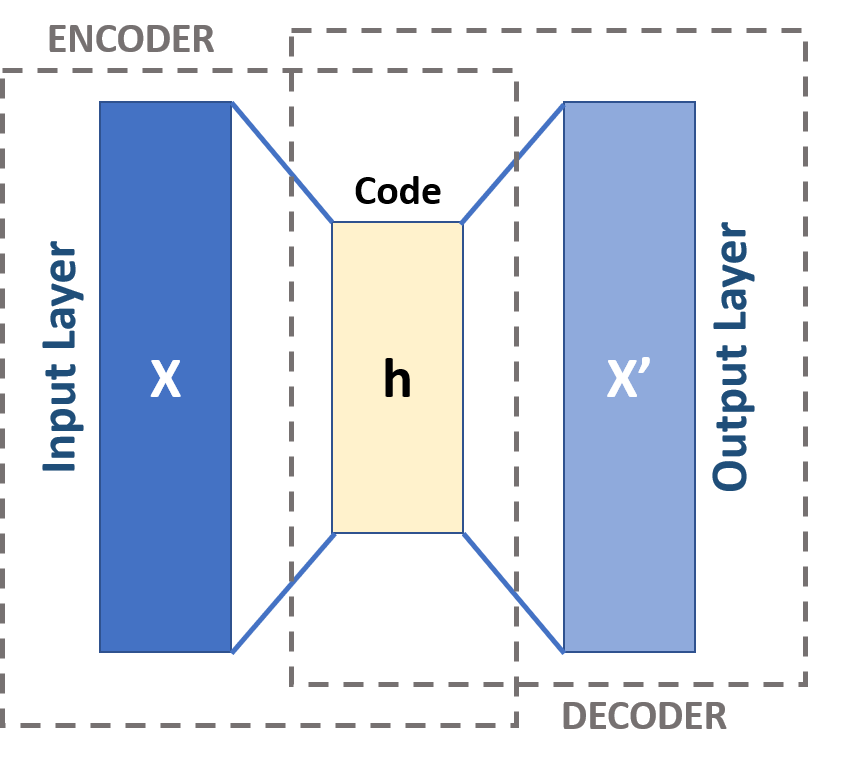
\includegraphics[width=0.3\textwidth]{../Images/autoencoder_schema.png}
   \centering
   \caption{Autoencoder schema \cite{wiki2019}}
   \label{fig:lstm_architecture}
  \end{figure}
  
 % subsection
 \subsection{CNN} \label{subsection::cnn}
  CNN (Convolutional neural network) is a type of network, which uses the mathematical operation convolution, instead of multiplication and addition.
  A CNN typically consists of three stages:
  \begin{enumerate}
   \item Convolutional operation
   \item Non-linearity (ReLU, sigmoid, $\ldots$)
   \item Pooling
  \end{enumerate}
  The convolutional operation used is more precisely a discrete convolutional operation.
  Convolutional operations are applicable on two or three dimensional data. As this thesis will always stick to image data, the equation is given for the
  two dimensional convolution. In general the network is useful for e.g. time-series, as they can be represented in two or three dimensional tensors and images.
  \begin{equation}
   (I \ast K)(i, j) = \sum_m\sum_nI(m,n)K(i-m,j-n)
  \end{equation}
  $I$ is the two dimensional image.\\
  $K$ is the two dimensional kernel.\\
  $\ast$ is the commonly used sign for the convolution operation.\\
  The first stage looks like:
  \begin{figure}[H]
   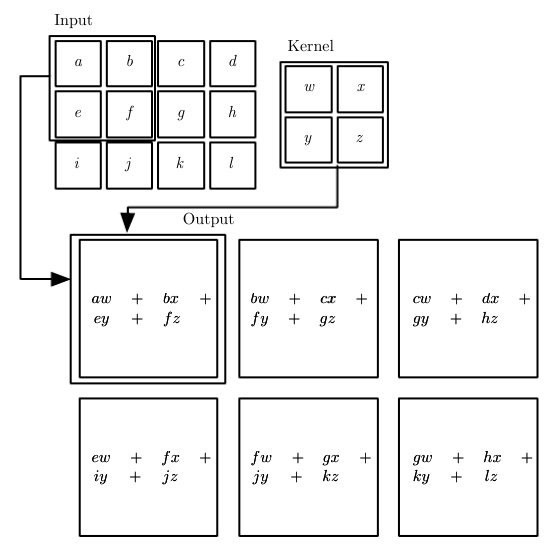
\includegraphics[width=0.35\textwidth]{../Images/kernel.png}
   \centering
   \caption{Two dimensional convolutional operation performed using a kernel \cite{Goodfellow2016}}
   \label{fig:kernel}
  \end{figure}\noindent
  In figure~\ref{fig:kernel}, one can see the idea of applying the kernel on the input data. In this example the stride is $0$ and the padding is $0$.\\
  The second stage is applying a non-linear function on the output, e.g. ReLU or simgoid.
  Lastly there is the pooling layer, in which a pooling function is applied on the output of the second stage. This is done to make the output of the second
  stage invariant to the input. The pooling layer reduces the output size by at least two. For example, an input image of size $(32 \times 32 \times 1)$,
  $(Height \times Width \times Channel)$ is then outputted at a maximum size of $(16 \times 16 \times 1)$.
  \begin{figure}[H]
   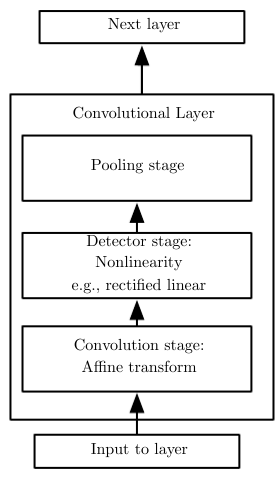
\includegraphics[width=0.25\textwidth]{../Images/convlayer.png}
   \centering
   \caption{Stages of a CNN \cite{Goodfellow2016}}
   \label{fig:cnn_stage}
  \end{figure}
  
 % subsection
 \subsection{RNN} \label{subsection::rnn}
  RNN (Recurrent neural network) is a network type, which is able to handle sequential data $X = (x_0, \ldots, x_{t-1})$, $|X| = t$. Therefore this type of network is used for e.g. time-series 
  analysis and image-/video-prediction~\ref{subsection::imageprediction}.\\\\
  Despite a standard feed-forward neural network, a RNN will not only get a new input at a time-step, but also the output
  of the RNN of the last time-step. This requires a RNN to be initialized at start, because there is no output of the last time-step available. This last time-step input is often initialized as $0$.
  A standard feed-forward neural network looks like:
  \begin{equation}
   \hat{y} = f_{\theta}(x)
  \end{equation}
  Every approximated output $\hat{y}$ is only dependent of the input $x$ and the computation inside the network.
  The RNN looks like:
  \begin{equation}
   \hat{y}^t = f_{\theta}(\hat{y}^{t-1};x^t) = f_{\theta}(f_{\theta}(\hat{y}^{t-2};x^{t-1});x^t) = \ldots
  \end{equation}
  The approximated output $\hat{y}^t$ depends on the input $x^t$, but also on all previous outputs.
  In the literature the RNN is often schemed using a folded and an unfolded graph, to illustrate how the network architecture works.
  \begin{figure}[H]
   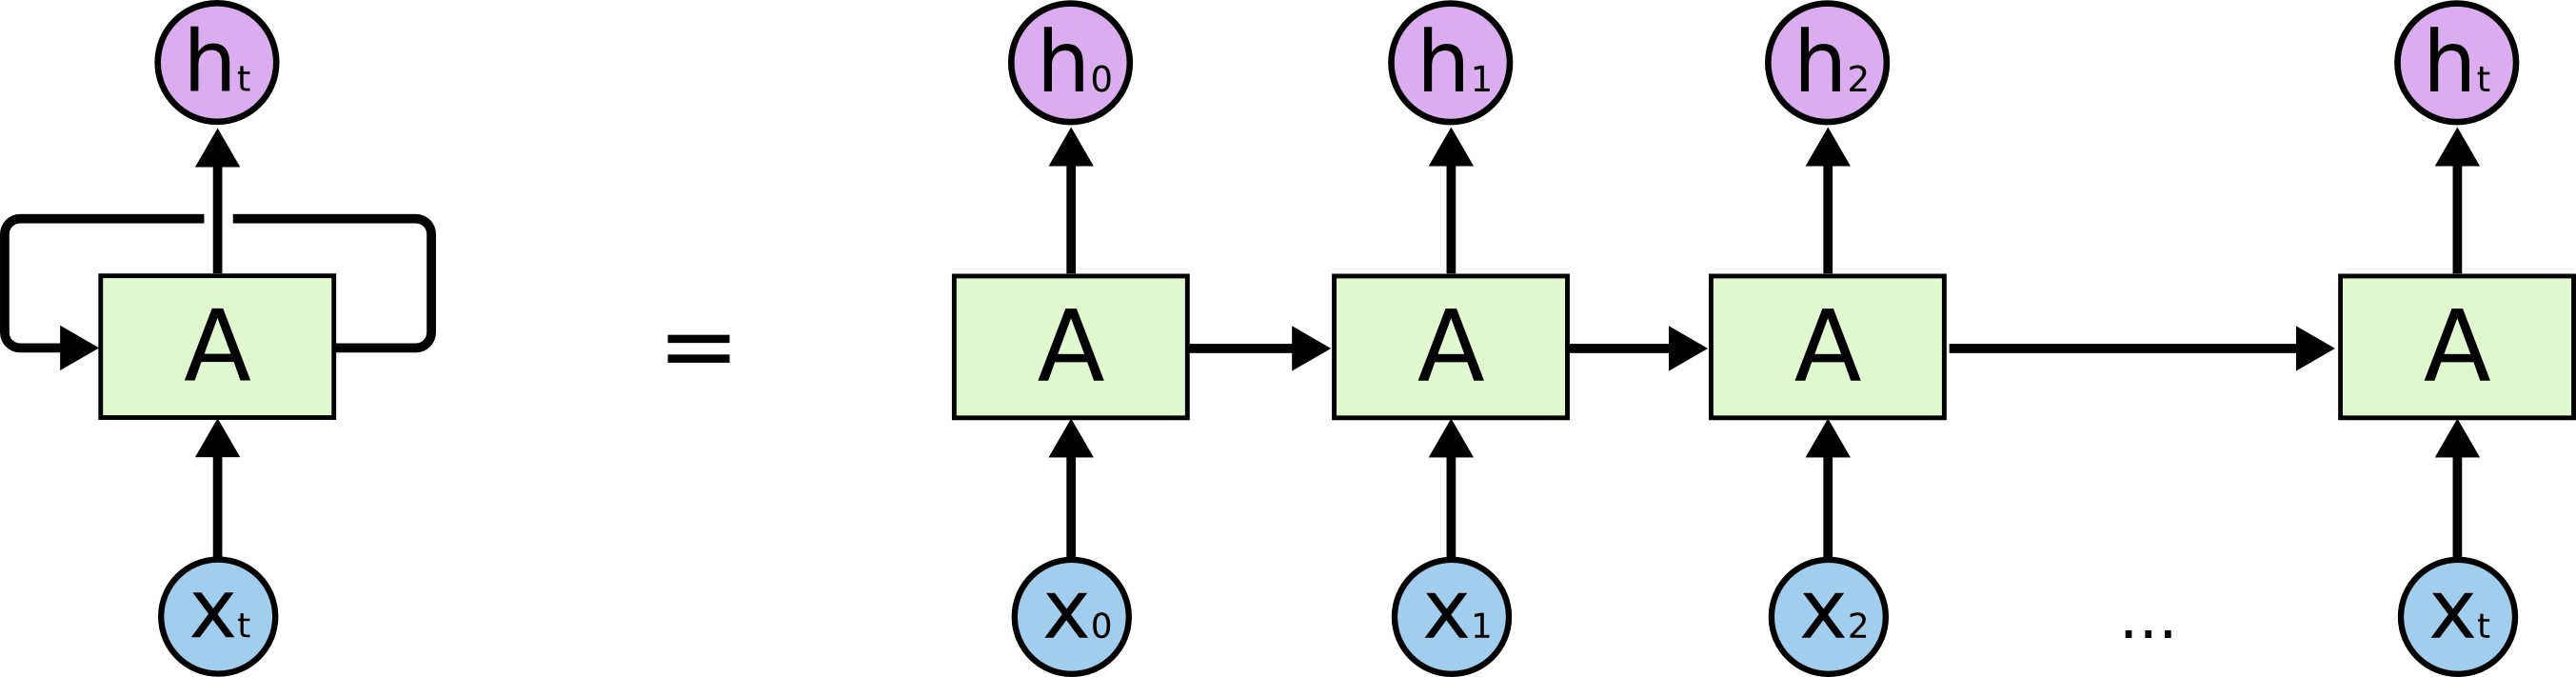
\includegraphics[width=0.8\textwidth]{../Images/rnn.png}
   \centering
   \caption{RNN schema. \textbf{Left:} Folded graph, \textbf{Right:} Unfolded graph \cite{Olah2015}}
   \label{fig:lstm_architecture}
  \end{figure}\noindent
  The output of a RNN is often denoted as $h$ for hidden-unit, because it is not only the output of the time-step, but also the input for the next time-step. \label{sentence::hidden}\\
  This networks are not learned with simple backpropagation~\ref{subsection::backpropagation}, but often with BPTT (Backpropagation through time)~\ref{subsection::bptt}.
 
 % subsection
 \subsection{LSTM} \label{subsection::lstm}
  LSTM (Long Short-term Memory), invented by Hochreiter and Schmidhuber \cite{Hochreiter1997} is a form of RNN, which avoids a critical problem of standard RNN: Saving 
  \textbf{Long-term dependencies} 
  \cite{Goodfellow2016}.
  The architecture consists of different submodules: An inpute-gate, forget-gate, cell-state and output-gate.
  \begin{equation}
   i_t = \sigma(w_{x_i}x_t + w_{h_i}h_{t-1} + b_i)
  \end{equation}
  \begin{equation}
   f_t = \sigma(w_{x_f}x_t + w_{h_f}h_{t-1} + b_f)
  \end{equation}
  \begin{equation}
   c_t = f_tc_{t-1} + i_ttanh(w_{x_c}x_t + w_{h_c}h_{t-1} + b_c)
  \end{equation}
  \begin{equation}
   o_t = \sigma(w_{x_o}x_t + w_{h_o}h_{t-1} + b_o)
  \end{equation}
  \begin{equation}
   h_t = o_ttanh(c_t)
  \end{equation}
  $w$ is the weight of the layer\\
  $\sigma$ the sigmoid function\\
  $b$ the layer bias.\\
  $h_t$ is the output, in RNN's the output is often denoted as hidden~\ref{sentence::hidden}.
  \begin{figure}[H]
   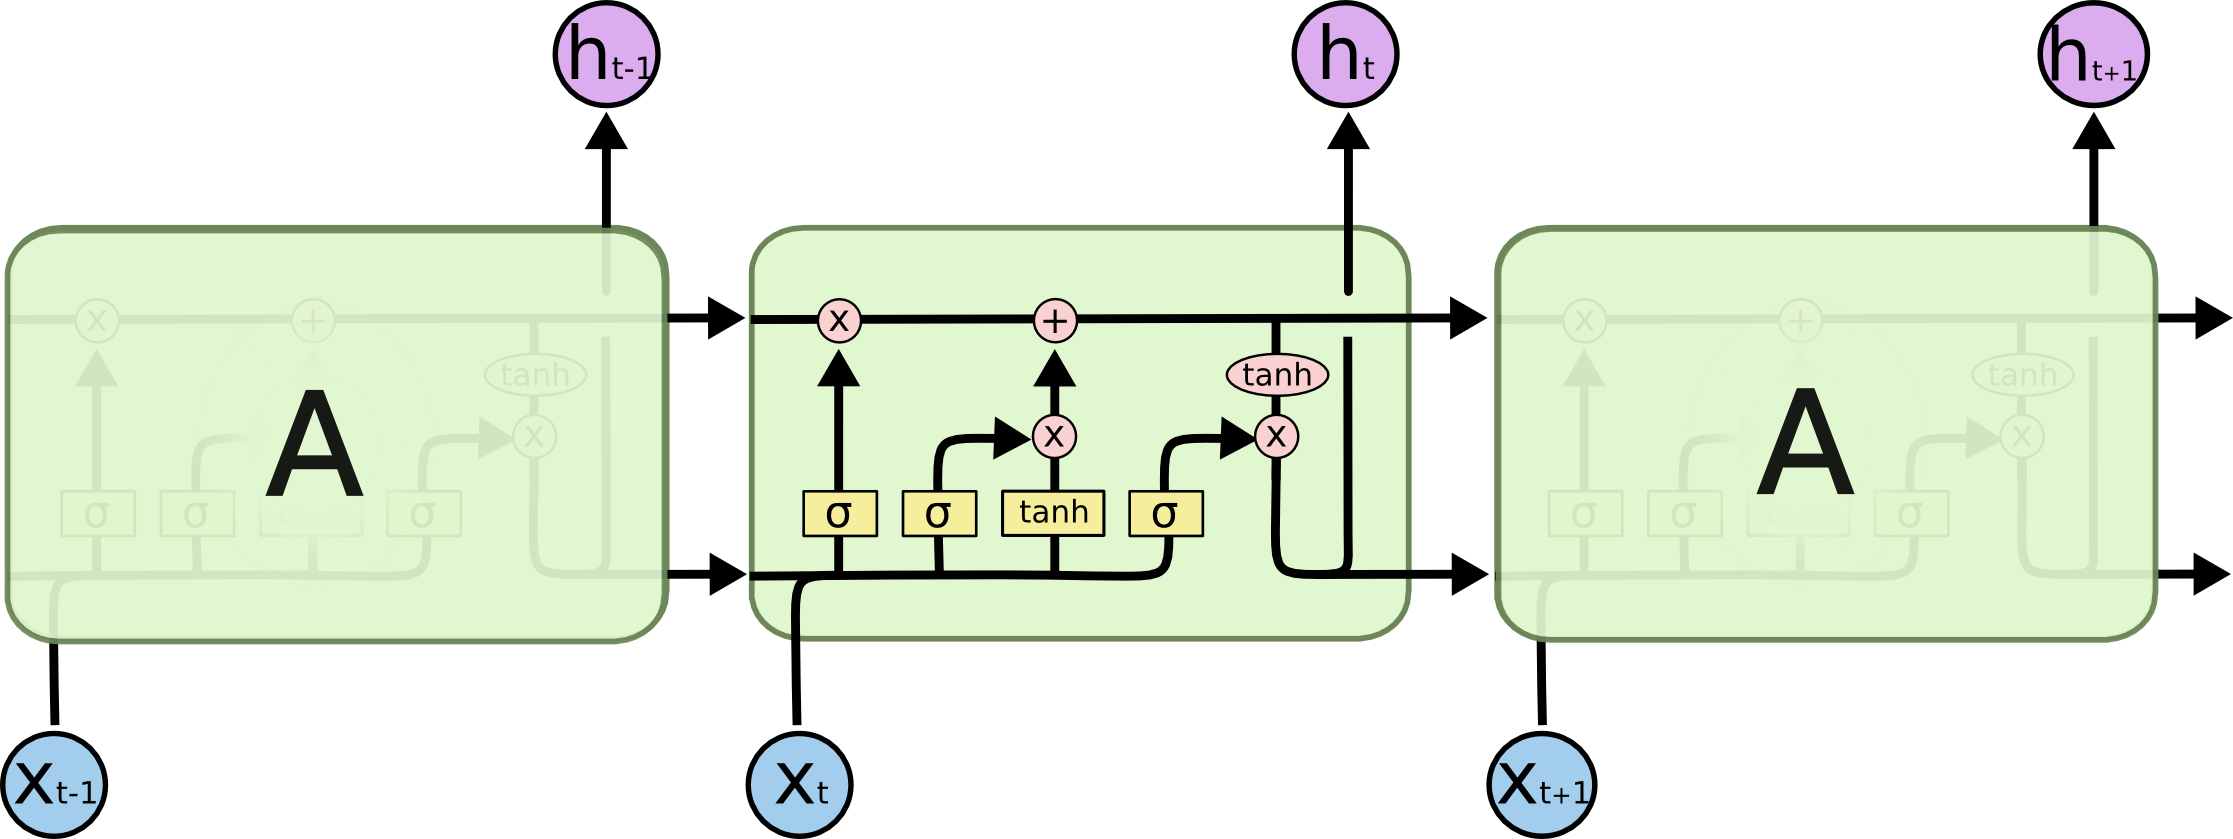
\includegraphics[width=0.7\textwidth]{../Images/lstm_chain.png}
   \centering
   \caption{LSTM Architecture \cite{Olah2015}}
   \label{fig:lstm_architecture}
  \end{figure}\noindent
  It is much better in saving long-term dependencies as a standard RNN, because of the cell-state. This cell-state can be seen as the main memory of the LSTM,
  where every iteration saves important information and deletes unnecessary information. The cell-state can be seen as the upper horizontal line in 
  figure~\ref{fig:lstm_architecture}.\\\\
  The given equations for the LSTM are for the very basic LSTM without peephole.\\
  The peephole is an idea from Gers and Schmidhuber from the year 2000 \cite{Gers2000}, where they augmented the LSTM
  with peephole connections, which gave them an advantage in learning spike trains\footnote[1]{Spike trains are time series of $0$s and $1$s, where $1$ is 
  defined as a spike.}, because a LSTM without peephole was not able to learn those spike trains.
  The equations looks very similar, with only few changes:
  \begin{equation}
   i_t = \sigma(w_{x_i}x_t + w_{c_i}c_{t-1} + b_i)
  \end{equation}
  \begin{equation}
   f_t = \sigma(w_{x_f}x_t + w_{c_f}c_{t-1} + b_f)
  \end{equation}
  \begin{equation}
   c_t = f_tc_{t-1} + i_ttanh(w_{x_c}x_t + b_c)
  \end{equation}
  \begin{equation}
   o_t = \sigma(w_{x_o}x_t + w_{c_o}c_t + b_o)
  \end{equation}
  \begin{equation}
   h_t = o_ttanh(c_t)
  \end{equation}
  
 % subsection
 \subsection{ConvLSTM} \label{subsection::convlstm}
  The convolutional LSTM, invented by Shi et. al. \cite{Shi2015} is a LSTM with peephole using convolutional layer instead of fully connected ones.
  Therefore the formulas look very similar to the ones in section~\ref{subsection::lstm}.
  \begin{equation}
   i_t = \sigma(x_t \ast w_{x_i} + h_{t-1} \ast w_{h_i} + w_{i_b})
  \end{equation}
  \begin{equation}
   f_t = \sigma(x_t \ast w_{x_f} + h_{t-1} \ast w_{h_f} + w_{f_b})
  \end{equation}
  \begin{equation}
   \tilde{c_t} = tanh(x_t \ast w_{x_{\tilde{c}}} + h_{t-1} \ast w_{h_{\tilde{c}}} + w_{c_{\tilde{b}}})
  \end{equation}
  \begin{equation}
   c_t = \tilde{c_t} \odot i_t + c_{t-1} \odot f_t
  \end{equation}
  \begin{equation}
   o_t = \sigma(x_t \ast w_{x_o} + h_{t-1} \ast w_{h_o} + w_{o_b})
  \end{equation}
  \begin{equation}
   h_t = o_t \odot tanh(c_t)
  \end{equation}
  $\ast$ is the commonly used sign for the convolution operation.\\
  $\odot$ is the hadamard product (point-wise multiplication).\\\\
  There is also a ConvLSTM without peephole, which is used in Patraucean et. al. \cite{Patraucean2015}, which is implemented in section~\ref{section::implementation}.
  
 % subsection
 \subsection{Backpropagation} \label{subsection::backpropagation}
  Backpropagation, invented in 1986 by Rumelhart et. al. \cite{Rumelhart1986}, is the most used algorithm for training neural networks, due to it's simplicity.
  The algorithm should be already known to the reader, therefore I will only give a very simple example of it at the most simple neural network, the Perceptron \cite{Rosenblatt1957}.
  \begin{center}
   \begin{tikzpicture}[roundnode/.style={circle, draw=green!60, fill=green!5, very thick, minimum size=7mm},
  					 roundnodesmall/.style={circle, draw=green!60, fill=green!5, thick, minimum size=1mm}]
    % Node
    \node[roundnode] (circle) {$\sum | \sigma$};
    \node[roundnodesmall] (x1) [above left=of circle] {$x_1$};
    \node[roundnodesmall] (x2) [below left=of circle] {$x_2$};
    \node[roundnodesmall] (y) [right=of circle] {$\hat{y}$};
    % Lines
    \draw[->, bend left=45] (x1.east) -- (circle) node[above left=1.2cm] {$w_1$};
    \draw[->] (x2.east) -- (circle) node[below left=1.2cm] {$w_2$};
    \draw[->] (circle) -- (y);
   \end{tikzpicture}
  \end{center}
  The usage of backpropagation is very straight forward. Neural networks are representation learning algorithms, which means, that they learn the representation of the data over time, without
  having the need of an expert doing supervision. It only needs a valid training and testing dataset, where one has ground-truth knowledge of the output of the data. One then leverages
  the forward pass of the algorithm to produce our approximated output.
  \begin{enumerate}
   \item \textbf{Forward pass:}
  \begin{equation}
   \hat{y} = \sigma(\sum_{i=1}^{2}x_iw_i)
  \end{equation}
  After computing the regarding output, one will compare the computed output with the ground-truth output with some kind of error-function, e.g. \textbf{MSE}:
  \begin{equation} \label{equation::mse}
   L(y,\hat{y}) = \frac{1}{N}||y-\hat{y}||_2^2 = \frac{1}{N}\sum_{i=1}^{N}(y_i-\hat{y}_i)^2
  \end{equation}    
  This error is then propagated back, using the chain-rule through the
  graph to update the weights of the network. This is done in the backward pass.\\
  \item \textbf{Backward pass:}
  \begin{equation}
   \frac{\partial L}{\partial \hat{y}} = \frac{2}{N}\sum_{i=1}^{N}(y_i-\hat{y}_i)
  \end{equation}
  \begin{equation} \label{equation::sigma_derivative}
   \frac{\partial \sigma(x)}{\partial x} = \sigma(x)(1-\sigma(x))
  \end{equation}
  \begin{equation}
   \frac{\partial L}{\partial \sum_{i=1}^{2}x_iw_i} = \frac{\partial L}{\partial \hat{y}} \cdot \frac{\partial \hat{y}}{\partial \sum_{i=1}^{2}x_iw_i} = \frac{2}{N}\sum_{i=1}^{N}(y_i-\hat{y}_i) \cdot
   \sigma(\sum_{i=1}^{2}x_iw_i)(1-\sigma(\sum_{i=1}^{2}x_iw_i))
  \end{equation}
  \begin{equation}
   \frac{\partial L}{\partial w_1} = \ldots = \frac{2}{N}\sum_{i=1}^{N}(y_i-\hat{y}_i) \cdot \sigma(\sum_{i=1}^{2}x_iw_i)(1-\sigma(\sum_{i=1}^{2}x_iw_i)) \cdot x_1
  \end{equation}
  \item \textbf{Update weights using Gradient Descent:}
  \begin{equation}
   w_1 = w_1^{old} - \lambda \cdot \frac{\partial L}{\partial w_1}
  \end{equation}
  $\lambda$ is the learning rate and is set as a hyperparameter.
  \end{enumerate}
  Those three steps are performed iterative, as long as the error value is higher then an artificially set value $\epsilon$.\\
  It is also useful to use a second derivative method e.g. Newton method, instead of Gradient Descent, but in most cases Gradient Descent is used,
  due to it's simplicity and parallelization properties \cite{Rumelhart1986}.
 
 % subsection
 \subsection{BPTT} \label{subsection::bptt}
  BPTT (Backpropagation through time), invented by Paul Werbos \cite{Werbos1990}, is a only slightly different algorithm, compared to simple backpropagation~\ref{subsection::backpropagation}.
  This algorithm is explicitly designed for RNN's and as the name already denotes, able to backpropagate through the time. To make it even more clear, the algorithm does nothing more, then
  unfolding the graph during the backward pass and backpropagates through all unfolded time-steps performed by the recurrent module. Let's make a simple example to fully understand the idea.
  Therefore I will use a simple RNN architecture found in Goodfellow \cite{Goodfellow2016}. To have a basic comparison to the backpropagation in section~\ref{subsection::backpropagation}, I changed
  the softmax function to $\sigma$, as this derivation is already known with equation~\ref{equation::sigma_derivative}.
  \begin{enumerate}
   \item \textbf{Forward pass:}
   \begin{equation}
    h_t = tanh(Wh_{t-1} + Ux_t + b_1)
   \end{equation}
   \begin{equation}
    o_t = Vh_t + b_2
   \end{equation}
   \begin{equation}
    \hat{y}_t = \sigma(o_t)
   \end{equation}
   $U,V,W$ are the weight matrices for input-to-hidden, hidden-to-output and hidden-to-hidden.\\
   After computing the output, one again needs an error function, e.g. MSE (known from equation~\ref{equation::mse}.)\\
   This time, it is also necessary to have this error function for every iteration.
   \begin{equation}
    L(y, \hat{y}) = \sum_{t}(L_t(y_t, \hat{y}_t))
   \end{equation}
   After computing the MSE for all time-steps and the overall error, one again starts the backward pass.
   \item \textbf{Backward pass:}
   \begin{equation}
    \frac{\partial L}{\partial V} = \sum_t\frac{\partial L_t}{\partial V}
   \end{equation}
   \begin{equation}
    \frac{\partial L_t}{\partial \hat{y}_t} = \frac{2}{N}\sum_{i=1}^{N}(y_t^i-\hat{y}_t^i)
   \end{equation}
   \begin{equation}
    \frac{\partial L_t}{\partial o_t} = \frac{\partial L_t}{\partial \hat{y}_t} \cdot \frac{\partial \hat{y}_t}{\partial o_t} = \frac{2}{N}\sum_{i=1}^{N}(y_t^i-\hat{y}_t^i) \cdot \sigma(o_t)(1-
    \sigma(o_t))
   \end{equation}
   \begin{equation}
    \frac{\partial L_t}{\partial V} = \frac{\partial L_t}{\partial \hat{y}_t} \cdot \frac{\partial \hat{y}_t}{\partial o_t} \cdot \frac{\partial o_t}{\partial V} = \frac{2}{N}\sum_{i=1}^{N}(y_t^i-
    \hat{y}_t^i) \cdot \sigma(o_t)(1-\sigma(o_t)) \cdot h_t
   \end{equation}
   \begin{equation}
    \frac{\partial L}{\partial V} = \sum_t\frac{\partial L_t}{\partial V}
   \end{equation}
   \item \textbf{Update weights using Gradient Descent:}
   \begin{equation}
    V = V^{old} - \lambda \cdot \frac{\partial L}{\partial V}
   \end{equation}
  \end{enumerate}
